\documentclass[]{article}
\usepackage{geometry}   % my added package "geometry"
\geometry{letterpaper,tmargin=1in,bmargin=1in,lmargin=2.2cm,rmargin=2.2cm}
\usepackage[colorlinks,bookmarksopen,bookmarksnumbered,
citecolor=green,urlcolor=red]{hyperref}
\hypersetup{pdfauthor={Name}}
%%%%%%%%%%%%%%%%%%%%%%%%%%%%%%%%%%%%%%%%%%%%%%%%%%%%%%%%%%%%%%%%%%%%%%%%%
%\usepackage{graphicx}
\usepackage{graphics}
\usepackage{epsfig}
\usepackage{epstopdf}
\usepackage{amsfonts}
\usepackage{amssymb}
\usepackage{booktabs}
\usepackage{color,soul}
%%%%%%%%%%%%%%%%%%%%%%%%%%%%%%%%%%%%%%%%%%%%%%%%%%%%%%%%%%%%%%%%%
\usepackage{amsmath}
\usepackage{cleveref}
\usepackage{authblk}
%\usepackage[fleqn]{amsmath}
\usepackage{lineno}
\usepackage{tikz}
\usepackage{standalone}
\usetikzlibrary{calc,patterns,arrows.meta,shapes.arrows,intersections,positioning}
\usetikzlibrary{decorations.pathmorphing,backgrounds,fit,petri}
\usepackage[percent]{overpic}
%%%%%%%%%%%%%%%%%%%%%%%%%%%%%%%%%%%%%%%%%%%%%%%%%%%%%%%%%%%%%%%%%
\usepackage{xcolor}
\usepackage{listings}
\lstset { %
	language=C++,
	backgroundcolor=\color{blue!5}, % set backgroundcolor
	basicstyle=\footnotesize\color{black},% basic font settingbasicstyle=\ttfamily\color{black}
	keywordstyle=\color{red},
	commentstyle=\color{violet},
	stringstyle=\color{blue},
	xleftmargin=2em,
	frame=single,
	framexleftmargin=2em,
	numbers=left,
	numberstyle=\tiny,
	numbersep=8pt,
}
%%%%%%%%%%%%%%%%%%%%%%%%%%%%%%%%%%%%%%%%%%%%%%%%%%%%%%%%%%%%%%%%%
\renewcommand\thesubsection{\thesection\Alph{subsection}}
%%%%%%%%%%%%%%%%%%%%%%%%%%%%%%%%%%%%%%%%%%%%%%%%%%%%%%%%%%%%%%%%%
\renewcommand\lstlistingname{Header}
\renewcommand\lstlistlistingname{Header}
%%%%%%%%%%%%%%%%%%%%%%%%%%%%%%%%%%%%%%%%%%%%%%%%%%%%%%%%%%%%%%%%%%%%
%opening
\begin{document}
\title{HiperLife Tutorial: NonLinear Thermal Conduction}
\author{Arash Imani}
\affil{LaCàN}
\maketitle

\linenumbers

\section{Problem Definition} \label{sec: pd}
Thermal conduction is the diffusion of thermal energy within one material or between materials in contact. Nowadays it is becoming more important to predict heat transport properties according to geometric structures or component materials which add complexity in form of nonlinearity to the PDEs. Here the simplest case of nonlinear heat transfer equation has been chosen to show how to use nonlinear solver within the time discretization.
\begin{figure}[htbp]
	\centering
	
\documentclass[preprint,12pt,a4]{standalone}
\usepackage{geometry}   % my added package "geometry"
\geometry{letterpaper,tmargin=1in,bmargin=1in,lmargin=2.5cm,rmargin=2.5cm}
\usepackage{tikz}
\usetikzlibrary{calc,patterns,arrows.meta,shapes.arrows,intersections,positioning}
\usetikzlibrary{decorations.pathmorphing,backgrounds,fit,petri}
\usepackage{standalone}
\begin{document}
	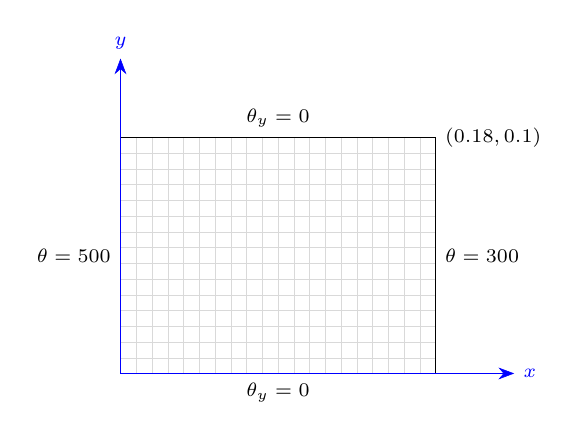
\begin{tikzpicture} [{place/.style={rectangle,draw=blue!50,fill=blue!20,ultra thin,inner sep=0.8mm}},{place2/.style={circle,draw=black!50,ultra thin,inner sep=0.8mm}},{linest/.style={color=gray,ultra thin}}]
	%%coordinates of corners of Beam
	\coordinate (A) at (0,0);
	\coordinate (B) at (2,0);
	\coordinate (C) at (4,0);
	\coordinate (D) at (4,1.5);
	\coordinate (E) at (4,3.0);
	\coordinate (F) at (2.0,3.0);
	\coordinate (G) at (0.0,3.0);
	\coordinate (H) at (0.0,1.5);
	%%mesh
	\draw [line width=0.1pt,gray!30,step=2mm](A) grid (E);
	%%Beam	
	\draw [color=black](A)-- (B)node [below,color = black,font=\scriptsize] {$\theta_y=0$}--(C)--(D)node [right,color = black,font=\scriptsize] {$\theta=300$}--(E)node [right,color = black,font=\scriptsize] {$(0.18,0.1)$}--(F)node [above,color = black,font=\scriptsize] {$\theta_y=0$}--(G)--(H)node [left,color = black,font=\scriptsize] {$\theta=500$}--(A);
	
	%%axes
	\draw [-{Stealth[length=2mm]},help lines,blue] (A) -> (5,0) node [right,color = blue,font=\scriptsize] {$x$};
		\draw [-{Stealth[length=2mm]}, help lines,blue] (A) -- (0,4) node [above,color = blue,font=\scriptsize] {$y$};

	\end{tikzpicture}
\end{document}
	\caption{Geometry, BC and computational domain used for the analysis of nonlinear heat transfer.}
	\label{fig_el}
\end{figure}
\section{Governing Equations} \label{sec: ge}
Consider the transient heat conduction equation \cite{reddy2014introduction}

\begin{equation}\label{eq1}
	\begin{aligned}
		\frac{\partial \theta}{\partial t} - \frac{\partial}{\partial x}(\kappa \frac{\partial\theta}{\partial x})- \frac{\partial}{\partial y}(\kappa \frac{\partial\theta}{\partial y}) = 0 \quad \text{in} \ \Omega\thinspace.
	\end{aligned}
\end{equation}

where $\theta$ is the temperature and $\kappa$ is the conductivity. as it is demonstrated in Figure \ref{fig_SB}, The domain $\Omega$ is a rectangle of dimensions $[1.18 \times 0.1]$ along the $x$ and $y$ coordinates, respectively; the conductivity $\kappa$ is of the form
\begin{equation}\label{eq2}
	\begin{aligned}
		\kappa = \kappa_0(1+\beta\theta)\thinspace.
	\end{aligned}
\end{equation}
where $\kappa_0=0.2 \ \text{W}/(m^{\ \circ}\text{C})$ and $\beta=2 \times 10^{-3 \ \circ}\text{C}^{-1}$.the boundary conditions to be
\begin{equation}\label{eq3}
	\begin{aligned}
		\theta(0,y,t) = 500^{ \ \circ}\text{C} , \quad \theta(0.18,y,t) = 300^{ \ \circ}\text{C}, \quad \theta_y(x,0,t) = \theta_y(x,0.1,t)=0\thinspace.
	\end{aligned}
\end{equation}
The initial condition is assumed to be
\begin{equation}\label{eq4}
	\begin{aligned}
		\theta(x,y,0) = 0\thinspace.
	\end{aligned}
\end{equation}

This is essentially a one-dimensional problem and $\Delta t = 0.005$ and we use Backward temporal approximation scheme.
\section{Weak Form} \label{sec: WF}
The starting point for the development of the finite element models of Eq. (\ref{eq1}) is their weak forms. By considering $\Delta t = t^{n+1} - t^{n}$, the $\alpha$-family approximation for the temperature field takes the following form
\begin{equation}\label{eq5}
	\begin{aligned}
		\{\theta\}^{n+1} = \{\theta\}^n + \Delta t(1 - \alpha)\{\theta_t\}^n + \Delta t\alpha\{\theta_t\}^{n+1}\thinspace.
	\end{aligned}
\end{equation}
The time derivatives of $\theta$ on the right hand side of this equation can be calculated from Eq. (\ref{eq1}) for each step, like this 
\begin{equation}\label{eq6}
	\begin{aligned}
		\{\theta_t\}^{n+1} &= \nabla(\kappa\nabla\{ \theta\}^{n+1})\thinspace, \\
		\{\theta_t\}^{n} &= \nabla (\kappa\nabla\{ \theta\}^{n})\thinspace. \
	\end{aligned}
\end{equation}
combining these two equations gives us
\begin{equation}\label{eq7}
	\begin{aligned}
		\{\theta\}^{n+1} -\Delta t\alpha[\nabla(\kappa \nabla\{\theta\}^{n+1})] - \{\theta\}^n - \Delta t(1 - \alpha)[\nabla(\kappa \nabla\{\theta\}^{n})]=0\thinspace.
	\end{aligned}
\end{equation}
The variation formulation of our model problem can be introduced as find $\theta \in V$ such that
\begin{equation}\label{eq8}
	\begin{aligned}
		\mathcal{F}(\theta;v) = 0 \quad \forall v \in \hat{V}\thinspace.
	\end{aligned}
\end{equation}
where
\begin{equation}\label{eq9}
	\begin{aligned}
		\mathcal{F}(\theta; v) =\int_{\Omega} v\{\theta\}^{n+1} -\Delta t\alpha v\nabla \cdot(\kappa \nabla\{ \theta\}^{n+1}) - v\{\theta\}^n - \Delta t(1 - \alpha)v\nabla \cdot(\kappa \nabla \{\theta\}^{n})\ \mathrm{d}\Omega \thinspace .
	\end{aligned}
\end{equation}
and
\begin{equation}\label{eq10}
	\begin{aligned}
		\hat{V} &= \{v \in H^1(\Omega) : v = 0 \text{ on } x=0\mbox{ and }x=0.18\}, \\
		V &= \{v \in H^1(\Omega) : v = 500 \text{ on } x=0\text{ and } v = 300\text{ on }x=0.18\}\thinspace.
	\end{aligned}
\end{equation}
The discrete problem arises as usual by restricting $V$ and $\hat{V}$ to a pair of discrete spaces.with $\theta = \sum_{j=1}^N \theta_j \phi_j$. Since $\mathcal{F}$ is a nonlinear function of $\theta$, the variational statement gives rise to a system of nonlinear algebraic equations. applying integration by part, Using Gauss’s theorem and also defining  heat flux density as $q_{\mathfrak{n}} =  [\nabla(\kappa\theta)]\cdot\mathfrak{n}$, the weak form takes the following form
\begin{equation}\label{eq11}
	\begin{aligned}
		\mathcal{F}(\theta; v) =& \int_{\Omega} v \{\theta\}^{n+1} + \Delta t \alpha\kappa\nabla v \nabla(\{ \theta\}^{n+1}) \ \mathrm{d} \Omega - \int_{\Omega} v\{\theta\}^{n} + \Delta t (1-\alpha) \kappa\nabla v \nabla(\{\theta\}^{n}) \ \mathrm{d} \Omega \\
		&- v \Delta t \int_{\Gamma}  \alpha v q^{n+1}_{\mathfrak{n}} + (1-\alpha)v q^{n}_{\mathfrak{n}} \ \mathrm{d} \Gamma\thinspace.
	\end{aligned}
\end{equation}
Applying boundary conditions ($\Gamma = \Gamma_N \cup \Gamma_D$):
\begin{equation}\label{eq12}
	\begin{aligned}
		v= 0 \quad &\text{ on } \Gamma_D\thinspace, \\
		\kappa\nabla [\theta] \cdot n = 0 \quad &\text{ on } \Gamma_N \thinspace.
	\end{aligned}
\end{equation}

we get the final form for $\mathcal{F}$
\begin{equation}\label{eq13}
	\begin{aligned}
		\mathcal{F}(\theta; v) =& \int_{\Omega} v \{\theta\}^{n+1} + \Delta t \alpha\kappa\nabla v \nabla(\{ \theta\}^{n+1}) \ d \Omega - \int_{\Omega} v\{\theta\}^{n} + \Delta t (1-\alpha) \kappa\nabla v\nabla(\{ \theta\}^{n}) \ \mathrm{d} \Omega\thinspace.
	\end{aligned}
\end{equation}
In order to linearize our discretized nonlinear PDE problem, we may use Newton’s method. which for the system $\mathcal{F}_i(\Theta_1,\ldots,\Theta_j)=0$ it can be formulated by the first terms of a Taylor series approximation for the value of the variational as
\begin{equation}\label{eq14}
	\begin{aligned}
		\sum_{j=1}^N {\partial \over\partial \Theta_j} \mathcal{F}_i(\Theta_1^k,\ldots,\Theta_N^k)\delta \Theta_j &= -\mathcal{F}_i(\Theta_1^k,\ldots,\Theta_N^k),\quad i=1, \ldots ,N,\\ \Theta_j^{k+1} &= \Theta_j^k + \delta \Theta_j,\quad j=1, \ldots ,N\thinspace.
	\end{aligned}
\end{equation}
where $k$ is an iteration index and $n$ is time step. An initial guess $\theta^0$ must be provided to start the algorithm.
We need to compute the $\partial \mathcal{F}_i/\partial \Theta_j$ and the right-hand side vector $-\mathcal{F}_i$. Our present problem has $\mathcal{F}_i$ given by above. the Hessian is given by
\begin{equation}\label{eq15}
	\begin{aligned}
		\mathcal{J}(\theta;v)= \int_{\Omega} v \frac{\partial \{\theta\}^{n+1}}{\partial \theta_j} + \Delta t \alpha  \nabla v \Bigg[\frac{\partial \kappa}{\partial \theta_j}\nabla \{\theta\}^{n+1} +  \kappa\nabla \frac{\partial \{\theta\}^{n+1}}{\partial \theta_j}\Bigg] \ \mathrm{d} \Omega
	\end{aligned}
\end{equation}
\section{Finite Element Model} \label{sec: fem}
Since we are developing the Ritz-Galerkin finite element model, the choice of the weight functions is restricted to the spaces of approximation functions used for the solution field. Suppose that the dependent variable $\theta$ approximated by expansions of the form
\begin{equation}\label{eq16}
	\begin{aligned}
		\theta(\mathbf{x}, t)= \sum_{m=1}^{M} \phi_m(\mathrm{x}) \mathbf{\theta}^m(t) = \boldsymbol{\Phi}^T\boldsymbol{\theta} \thinspace,
	\end{aligned}
\end{equation}
Lets rewrite this equation for known and unknown variables.
\begin{equation}\label{eq17}
	\begin{aligned}
		\mathcal{J}(\theta;\phi)&= \int_{\Omega} \phi \phi^T + \Delta t \alpha \kappa_0 \nabla \phi \Big[\beta \phi^T \nabla \{\theta\} ^{n+1} + (1+\beta \{\theta\}^{n+1}) \nabla \phi^T\Big]\mathrm{d} \Omega\thinspace.
	\end{aligned}
\end{equation}

The above equations can be written symbolically in matrix form as we are going to solve it, 
\begin{equation}\label{eq18}
	\begin{aligned}
		\sum_j \mathcal{J}(\theta;\phi)\{\delta \theta_j\}^{n+1} = -\mathcal{F}(\theta;\phi)\thinspace.
	\end{aligned}
\end{equation}
where $\mathcal{F}(\theta;\phi)$ is
\begin{equation}\label{eq19}
	\begin{aligned}
		\mathcal{F}(\theta;\phi)= \int_{\Omega} \phi \{\theta\}^{n+1} + \kappa_0 \Delta t \alpha (1+\beta \{\theta\}^{n+1})\nabla \phi \nabla \{\theta\}^{n+1} - \phi \theta^{n} + \kappa_0 \Delta t \alpha (1+\beta \{\theta\}^{n})\nabla \phi \nabla \{\theta\}^{n}\mathrm{d} \Omega\thinspace.
	\end{aligned}
\end{equation}
The elemental representation of the vector and matrix required for filling function in hiperlife would be like
\begin{equation}\label{eq20}
	\begin{aligned}[b]
		Ak (i,j) =& jac \times \Big[\phi_i \phi_j + \Delta t \alpha \kappa_0 \nabla \phi_i \Big(\beta \phi_j \nabla \{\theta\} ^{n+1} + (1+\beta \{\theta\}^{n+1}) \nabla \phi_j\Big)\Big]\thinspace, \\
		Bk (i) =& jac \times \Big[\phi_i \{\theta\}^{n+1} + \kappa_0 \Delta t \alpha (1+\beta \{\theta\}^{n+1})\nabla \phi_i \nabla \{\theta\}^{n+1} - \phi_i \theta^{n} + \kappa_0 \Delta t \alpha (1+\beta \{\theta\}^{n})\nabla \phi_i \nabla \{\theta\}^{n}\Big]\thinspace.
	\end{aligned}
\end{equation}
Note that $\mathrm{d}A=\mathrm{d}x_{1} \times \mathrm{d}x_{2}=jac \ \mathrm{d}\xi \mathrm{d}\eta$, which $jac=\mathrm{det}(Jacobian)$.
\section{Choice of Elements} \label{sec: coe}
Thus, for this simple problem every Lagrange and serendipity family of interpolation functions are admissible for the interpolation of the temperature field, our choice is would be quadratic quadrilateral elements consist of $9$ nodes. The shape function with respect to the reference element are given for the vertex nodes ($I = 1, 2, 3, 4$):
\begin{equation}\label{eq21}
	\begin{aligned}[b]
		\boldsymbol{\Phi}_{I}(\xi, \eta) = \frac{1}{4}(\xi^2+\xi_I\xi)(\eta^2+\eta_I\eta)
	\end{aligned}
\end{equation}
-the middle edge nodes ($I = 5, 6, 7, 8$):
\begin{equation}\label{eq22}
	\begin{aligned}[b]
		\boldsymbol{\Phi}_{I}(\xi, \eta) = \frac{1}{2}\xi_I^2(\xi^2+\xi_I\xi)(1-\eta^2) + \frac{1}{2}\eta_I^2(\eta^2+\eta_I\eta)(1-\xi^2)
	\end{aligned}
\end{equation}
-and the middle node ($I = 9$):
\begin{equation}\label{eq23}
	\begin{aligned}[b]
		\boldsymbol{\Phi}_{I}(\xi, \eta) = (1-\xi^2)(1-\eta^2)
	\end{aligned}
\end{equation}
where $\xi_{I}$ and $\eta_{I}$ are the corner coordinates at element $T$ in domain of $\Omega_{T} \in (-1,1)^2$. As it shown in Figure \ref{fig_el} we are using $2 \times 2$ Gauss–Legendre quadrature integration.
\begin{figure}[htbp]
	\centering
	\documentclass[preprint,12pt,a4]{standalone}
\usepackage{geometry}   % my added package "geometry"
\geometry{letterpaper,tmargin=1in,bmargin=1in,lmargin=2.5cm,rmargin=2.5cm}
\usepackage{tikz}
\usetikzlibrary{calc,patterns,arrows.meta,shapes.arrows,intersections,positioning}
\usetikzlibrary{decorations.pathmorphing,backgrounds,fit,petri}
\usepackage{standalone}
%
\begin{document}
	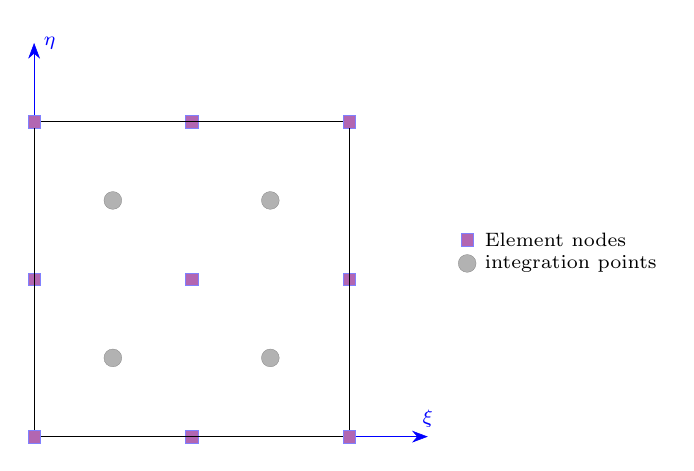
\begin{tikzpicture} [{place/.style={rectangle,draw=blue!50,fill=blue!20,ultra thin,inner sep=0.8mm}},{place2/.style={circle,draw=black!50,ultra thin,inner sep=0.8mm}},{linest/.style={color=gray,ultra thin}}]
		%axes
		\draw [{Stealth[length=2mm]}-{Stealth[length=2mm]}, help lines,blue] (5.0,0)node[above,font=\scriptsize]{$\xi$} -- (0.0,0.0) -- (0.0,5.0)node[right,font=\scriptsize] {$\eta$};
		%%element nodes
		\node at (0.0,0.0) [place,fill=violet!60] (1) {};
		\node at (4.0,0.0) [place,fill=violet!60] (2) {};
		\node at (4.0,4.0) [place,fill=violet!60] (3) {};
		\node at (0.0,4.0) [place,fill=violet!60] (4) {};
		\node at (2.0,0.0) [place,fill=violet!60] (5) {};
		\node at (4.0,2.0) [place,fill=violet!60] (6) {};
		\node at (2.0,4.0) [place,fill=violet!60] (7) {};
		\node at (0.0,2.0) [place,fill=violet!60] (8) {};
		\node at (2.0,2.0) [place,fill=violet!60] (9) {};
		
		%% integration points
	    \node at (1.0,1.0) [place2,fill=gray!60] (10) {};
		\node at (3.0,1.0) [place2,fill=gray!60] (11) {};
		\node at (1.0,3.0) [place2,fill=gray!60] (12) {};
		\node at (3.0,3.0) [place2,fill=gray!60] (13) {};
		%%element border
		\draw [-,black] (1) -- (2) -- (3) -- (4) --(1);
		%%middle nodes
		\node at (5.6,2.5) [right,font=\scriptsize]{$\mathrm{Element \ nodes}$};
		\node at (5.5,2.5) [place,fill=violet!60] (4) {};
		\node at (5.6,2.2) [right,font=\scriptsize]{$\mathrm{integration \ points}$};
		\node at (5.5,2.2) [place2,fill=gray!60] (4) {};
		
	\end{tikzpicture}
\end{document}
	\caption{Quadratic quadrilateral element used for finite element model.}
	\label{fig_el}
\end{figure}
We also chose a uniform mesh of size $10 \times 10$ to model the domain of our problem.
\section{Implementation} \label{sec: imp}
In this section, we present the implementation of our solution in the Hiperlife. The program is divided into three separate files, main part which we create our problem by the Hiperlife headers, auxiliary header where we introduce parameters and declare defined functions, and at last auxiliary file, where we define some functions which provide required matrices like the Jacobian and the Hessian.
\subsubsection{HeatTransferNonL.cpp} \label{sec: m.cpp}
\nolinenumbers
\begin{lstlisting}
/*
* Heat Transfer conduction nonlinear
*/
// cpp headers
#include <iostream>
#include <fstream>
#include <cmath>

// hiperlife headers
#include "hl_Core.h"
#include "hl_ParamStructure.h"
#include "hl_Parser.h"
#include "hl_TypeDefs.h"                                      
#include "hl_GlobalBasisFunctions.h"
#include "hl_StructMeshGenerator.h"         
#include "hl_DistributedMesh.h"                                           
#include "hl_FillStructure.h"
#include "hl_DOFsHandler.h"
#include "hl_SurfLagrParam.h"
#include "hl_HiPerProblem.h"
#include "hl_LinearSolver_Iterative_AztecOO.h"
#include "hl_NonlinearSolver_NewtonRaphson.h"
#include <hl_ConsistencyCheck.h>

// Header to auxiliary functions
#include "AuxHeatTransferNonL.h"

// -------------------------------------------------------------------//
/// -----------------   MAIN FUNCTION     --------------------------///
// -------------------------------------------------------------------//

int main(int argc, char** argv)
{
	using namespace std;
	using namespace hiperlife;
	using namespace hiperlife::Tensor;
	
	// ---------------------------------------------------------------//
	/// *****                 INITIALIZATION                    *****///
	// ---------------------------------------------------------------//
	
	// Initialize MPI
	hiperlife::Init(argc, argv);
	
	// ---------------------------------------------------------------//
	/// *****                   DATA INPUT                      *****///
	// ---------------------------------------------------------------//
	// Time-related parameters
	int maxSteps = 1000;
	double maxTime  = 0.1;
	double maxDeltat = 1.0;
	double adaptiveFactor = 1.;
	
	// number of output files 
	int nSave = 10;
	
	// Put parameters in the user structure
	SmartPtr<ParamStructure> paramStr = CreateParamStructure<HeatParams>();
	
	// Data
	paramStr->setRealParameter(HeatParams::delta_t, 0.005);
	paramStr->setRealParameter(HeatParams::alpha, 0.5);
	double delta_t = paramStr->getRealParameter(HeatParams::delta_t);
	
	// ---------------------------------------------------------------//
	/// *****                   MESH CREATION                   *****///
	// ---------------------------------------------------------------//
	
	// Create a rectangular structured mesh       
	SmartPtr<StructMeshGenerator> structMesh = Create<StructMeshGenerator>();
	structMesh->setNDim(3);
	structMesh->setBasisFuncType(BasisFuncType::Lagrangian);
	structMesh->setBasisFuncOrder(2);
	structMesh->setElemType(ElemType::Square);
	structMesh->genRectangle(4, 2, 0.18, 0.1);
	
	// Distributed mesh
	SmartPtr<DistributedMesh> disMesh = Create<DistributedMesh>();
	disMesh->setMesh(structMesh);
	disMesh->setBalanceMesh(true);
	disMesh->setElementLocatorEngine(ElementLocatorEngine::BoundingVolumeHierarchy);
	disMesh->Update();
	
	// checking mesh
	disMesh->printFileLegacyVtk("mesh");
	
	// ---------------------------------------------------------------//
	/// *****               DOFsHANDLER CREATION                *****///
	// ---------------------------------------------------------------//
	
	// DOFHandler
	SmartPtr<DOFsHandler> dofHand = Create<DOFsHandler>(disMesh);
	dofHand->setNameTag("dofHand");
	dofHand->setNumDOFs(1);
	dofHand->setDOFs({"theta"});
	dofHand->Update();
	// ------------------ Initial conditions------------------------ //
	//---------------------------------------------------------------//
	double f;
	for (int i = 0; i < disMesh->loc_nPts(); i++)
	{
		// Coordinate
		std::vector<double> x = disMesh->nodeCoords(i, IndexType::Local);
		f = 0.0 * x[i];
		// Initial condition
		dofHand->nodeDOFs->setValue("theta", i, IndexType::Local, f);
		// ---------------------- Boundary condition ---------------- //
		//------------------------------------------------------------//
		if (x[0] < 1e-5)
		{
			dofHand->nodeDOFs->setValue("theta", i, IndexType::Local,500.0);
			dofHand->setConstraint("theta",i, IndexType::Local,0.0);
		}
		if (x[0] > (0.18-1e-5))
		{
			dofHand->nodeDOFs->setValue("theta", i, IndexType::Local,300.0);
			dofHand->setConstraint("theta",i, IndexType::Local,0.0);
		}
	}
	// Update
	dofHand->nodeDOFs0->setValue(dofHand->nodeDOFs);
	dofHand->nodeDOFs0->UpdateGhosts();
	dofHand->UpdateGhosts();
	// checking initial and boundary condition
	dofHand->printFileLegacyVtk("HeatTransferNonL0");
	// ---------------------------------------------------------------//
	/// *****               HIPERPROBLEM CREATION               *****///
	// ---------------------------------------------------------------//
	
	SmartPtr<HiPerProblem> hiperProbl = Create<HiPerProblem>();
	hiperProbl->setParameterStructure(paramStr);
	hiperProbl->setDOFsHandlers({dofHand});
	hiperProbl->setIntegration("Integ", {"dofHand"});
	hiperProbl->setCubatureGauss("Integ", 4);
	hiperProbl->setElementFillings("Integ", LS);
	if (true)
	{
		hiperProbl->setConsistencyDOFs("dofHand", {"theta"});
		hiperProbl->setElementFillings("Integ", ConsistencyCheck<LS>);
		hiperProbl->setConsistencyCheckType(ConsistencyCheckType::Hessian);
	}
	hiperProbl->Update();
	
	// ---------------------------------------------------------------//
	/// *****                  SOLVER CREATION                  *****///
	// ---------------------------------------------------------------//
	
	SmartPtr<AztecOOIterativeLinearSolver> linsolver= 
	Create<AztecOOIterativeLinearSolver>();
	linsolver->setHiPerProblem(hiperProbl);
	linsolver->setTolerance(1.E-8);
	linsolver->setMaxNumIterations(500);
	linsolver->setSolver(AztecOOIterativeLinearSolver::Solver::Gmres);
	linsolver->setPreconditioner(AztecOOIterativeLinearSolver::Preconditioner::None);
	linsolver->setDefaultParameters();
	linsolver->setVerbosity(AztecOOIterativeLinearSolver::Verbosity::None);
	linsolver->Update();
	
	// Create nonlinear solver
	SmartPtr<NewtonRaphsonNonlinearSolver> nonLinSolver = 
	Create<NewtonRaphsonNonlinearSolver>();
	nonLinSolver->setLinearSolver(linsolver);
	nonLinSolver->setConvRelTolerance(true);
	nonLinSolver->setMaxNumIterations(15);
	nonLinSolver->setResTolerance(1e-6);
	nonLinSolver->setSolTolerance(1e-6);
	nonLinSolver->setResMaximum(1e5);
	nonLinSolver->setSolMaximum(1e5);
	nonLinSolver->setExitRelMaximum(true);
	nonLinSolver->setLineSearch(false);
	nonLinSolver->setPrintSummary(false);
	nonLinSolver->setPrintIntermInfo(true);
	nonLinSolver->Update();
	// ---------------------------------------------------------------//
	/// *****                SOLVE HIPERPROBLEM                 *****///
	// ---------------------------------------------------------------//
	// Load loop
	int timeStep{1};
	double time{delta_t};
	double delta_t0 = delta_t;
	while (timeStep <= maxSteps and time <= maxTime)
	{
		// Print info
		if (hiperProbl->myRank() == 0)
		cout<<endl<<endl<<"Time step:"<<timeStep<<"/"<<maxSteps<<"deltat"<<delta_t
		<<"time"<<time<<"/"<<maxTime<<endl;
		
		paramStr->setRealParameter(HeatParams::delta_t,delta_t);
		paramStr->setRealParameter(HeatParams::time,time);
		paramStr->setIntParameter(HeatParams::timeStep,timeStep);
		// Initial guess
		dofHand->nodeDOFs->setValue(dofHand->nodeDOFs0);
		hiperProbl->UpdateGhosts();
		
		bool converged = nonLinSolver->solve();
		
		// Check convergence
		if (converged)
		{
			// Save solution
			dofHand->nodeDOFs0->setValue(dofHand->nodeDOFs);
			dofHand->nodeDOFs0->UpdateGhosts();
			
			// Save results each nSave time steps
			if (timeStep%2 == 0)  
			{
				// Output results
				string solName = "CondNL." + to_string(timeStep);
				dofHand->printFileLegacyVtk(solName,true);
			}
			
			// Update load variables
			timeStep++;
			int iter = nonLinSolver->numberOfIterations();
			if (iter < 4)
			delta_t /= adaptiveFactor;
			else if (iter == 5)
			delta_t *= adaptiveFactor;
			if (delta_t > maxDeltat)
			delta_t = maxDeltat;
			if (time < maxTime && time + delta_t >= maxTime)
			delta_t = maxTime - time;
			time += delta_t;
		}
		else
		{
			// End if no adaptivity
			if (adaptiveFactor == 1.0)
			{
				cout << endl << endl<< "Not converged" << endl;
				break;
			}
			
			// Steady state or non-convergence
			if (delta_t < 1e-8)
			{
				cout <<endl<<endl<<"Steady state or non-convergence"<<endl;
				break;
			}
			time -=delta_t;
			delta_t *= adaptiveFactor;
			time += delta_t;
		}
	}
	hiperlife::Finalize();
	return 0;
}

\end{lstlisting}
\subsubsection{AuxHeatTransferNonL.h} \label{sec: a.h}
\begin{lstlisting}
#ifndef AUXHeat_H
#define AUXHeat_H

// C headers
#include <iostream>

// hiperlife headers
#include "hl_Core.h"
#include "hl_ParamStructure.h"
#include "hl_Parser.h"
#include "hl_TypeDefs.h"                                                                         
#include "hl_GlobalBasisFunctions.h"                             
#include "hl_StructMeshGenerator.h"                                                                             
#include "hl_DistributedMesh.h"                                           
#include "hl_FillStructure.h"                                             
#include "hl_DOFsHandler.h"          
#include "hl_HiPerProblem.h"
#include "hl_SurfLagrParam.h"
#include "hl_LinearSolver_Iterative_AztecOO.h"
#include "hl_NonlinearSolver_NewtonRaphson.h"

// alpha = 0.5: crank nicolson; delta_t = 0.05
// alpha = 1: backward euler; delta_t = 0.05
struct HeatParams
{
	enum RealParameters
	{
		delta_t,
		time,
		alpha,
	};
	enum IntParameters
	{   
		timeStep,
	};
	HL_PARAMETER_LIST DefaultValues
	{
		{"delta_t,", 0.005},
		{"time,", 0.005},
		{"alpha,", 0.5},
		{"timeStep", 0},
	};
};

void LS(hiperlife::FillStructure& fillStr);

#endif

\end{lstlisting}
\subsubsection{AuxHeatTransferNonL.cpp} \label{sec: a.cpp}
\begin{lstlisting}
// Header to auxiliary functions
#include "AuxHeatTransferNonL.h"

// Hiperlife headers
#include "hl_Core.h"
#include "hl_ParamStructure.h"
#include "hl_Parser.h"
#include "hl_TypeDefs.h"                                                                         
#include "hl_GlobalBasisFunctions.h"                             
#include "hl_StructMeshGenerator.h"                                                                             
#include "hl_DistributedMesh.h"                                           
#include "hl_FillStructure.h"                                             
#include "hl_DOFsHandler.h"          
#include "hl_HiPerProblem.h"
#include "hl_SurfLagrParam.h"    
#include "hl_LinearSolver_Iterative_AztecOO.h"
#include "hl_NonlinearSolver_NewtonRaphson.h"

using namespace std;
using namespace hiperlife;
using namespace hiperlife::Tensor;


// Conduction

void LS(hiperlife::FillStructure& fillStr)
{
	double alpha  = fillStr.getRealParameter(HeatParams::alpha);
	double delta_t = fillStr.getRealParameter(HeatParams::delta_t);
	double k0{0.2};
	double beta{0.002};
	
	//---------------------------------------------------------------------------//
	// ------------------------------- INPUT DATA -------------------------------//
	//---------------------------------------------------------------------------//
	
	// Dimensions
	SubFillStructure& subFill = fillStr["dofHand"];
	int nDOFs = subFill.numDOFs;                                        
	int eNN   = subFill.eNN;                                           
	int nDim  = subFill.nDim;                                        
	int pDim  = subFill.pDim;
	
	// Nodal values at Gauss points
	wrapper<double,1> nborDOFs(subFill.nborDOFs.data(),eNN);
	wrapper<double,1> nborDOFs0(subFill.nborDOFs0.data(),eNN);
	
	// Shape functions and derivatives at Gauss points
	double jac;
	wrapper<double,1>  bf(subFill.nborBFs(), eNN); //basis function
	tensor<double,2> Dbf(eNN,pDim);                //gradient of basis function
	GlobalBasisFunctions::gradients(Dbf, jac, subFill);
	
	//-------------------------------------------------------------------------------//
	// --------------------- Initializing Hessian & Jacobian ------------------------//
	//-------------------------------------------------------------------------------//
	wrapper<double,2> Ak(fillStr.Ak(0, 0).data(), eNN, eNN);
	wrapper<double,1> Bk(fillStr.Bk(0).data(),eNN);
	
	//-------------------------------------------------------------------------------//
	// -------------------------------- VARIABLES -----------------------------------//
	//-------------------------------------------------------------------------------//
	
	// temp
	double theta = product(bf, nborDOFs, {{0, 0}});
	double theta0 = product(bf, nborDOFs0, {{0, 0}});
	
	// Temperature Gradient
	tensor<double, 1> grad_t = product(Dbf, nborDOFs, {{0,0}});
	tensor<double, 1> grad_t0 = product(Dbf, nborDOFs0, {{0,0}});
	
	// (bf) * (bf)
	tensor<double, 2> bfbf = outer(bf, bf);
	
	// (gradient of the bf) *  (gradient of the bf)
	tensor<double, 2> DbfDbf = product(Dbf, Dbf, {{1, 1}});
	
	// (gradient of the bf) *  (gradient of t)
	tensor<double, 1> DtDbf = product(grad_t, Dbf, {{0, 1}});
	tensor<double, 1> Dt0Dbf = product(grad_t0, Dbf, {{0, 1}});
	tensor<double, 2> bfDbf = outer(DtDbf, bf);
	//-------------------------------------------------------------------------------//
	//----------------------- Filling Hessain and Jacobian --------------------------//
	//-------------------------------------------------------------------------------// 
	
	Bk += jac * (bf*theta + delta_t*alpha*k0*(1.0 + beta*theta)*DtDbf -
	             bf*theta0 + delta_t*(1.0-alpha)*k0*(1.0 + beta*theta0)*Dt0Dbf);
	Ak += jac * (bfbf + k0*delta_t*alpha*(beta*bfDbf + (1.0 + beta*theta)*DbfDbf));
}


\end{lstlisting}

\section{Results} \label{sec: rst}
In this section, we present the results of our solution. The contour demonstration of temperature in the whole domain is shown in Figure \ref{fig_Rs2}.
\begin{figure}[htbp]
	\centering
	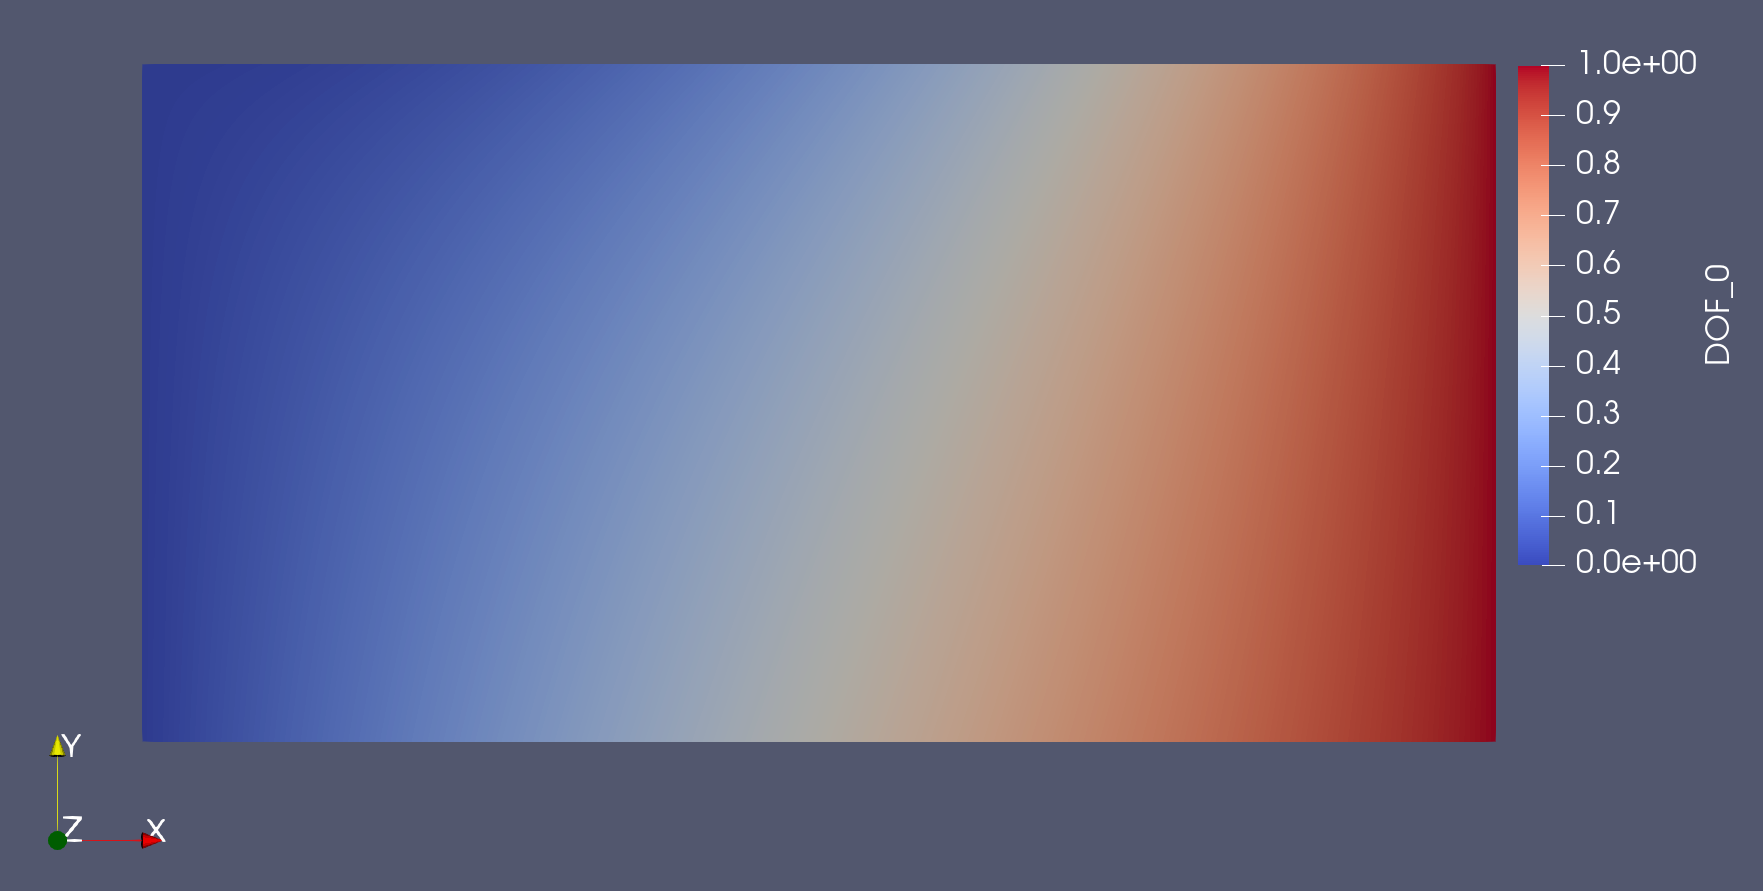
\includegraphics[width=0.6\textwidth]{Figures/result.png}
	\caption{Distrobution of $\theta$ in the problem domain.}
	\label{fig_Rs2}
\end{figure}
\bibliographystyle{unsrt}
\bibliography{ref} 
\end{document}
